\documentclass[conference]{IEEEtran}
\IEEEoverridecommandlockouts
\usepackage{cite}
\usepackage{amsmath,amssymb,amsfonts}
\usepackage{graphicx}
\usepackage{textcomp}
\usepackage{xcolor}
\usepackage{booktabs}
\usepackage{tikz}
\usetikzlibrary{arrows.meta, positioning, fit, backgrounds, calc}
\usepackage{hyperref}
\usepackage{listings}
\usepackage{caption}

\lstset{
  basicstyle=\ttfamily\scriptsize,
  breaklines=true,
  columns=fullflexible,
  frame=single,
  backgroundcolor=\color{gray!8}
}

\def\BibTeX{{\rm B\kern-.05em{\sc i\kern-.025em b}\kern-.08em
    T\kern-.1667em\lower.7ex\hbox{E}\kern-.125emX}}

\begin{document}

\title{TrustShield AI: A Hybrid Trust Layer for Explainable Verification of\\
Retrieval-Augmented Language Model Responses}

\author{
\IEEEauthorblockN{Shivam Shaurya}
\IEEEauthorblockA{\textit{Department of Computer Science} \\
\textit{B.Tech Project (BTP)} \\
India \\
shivam.shaurya@rodicconsultants.com}
}

\maketitle

\begin{abstract}
Large language models (LLMs) produce fluent text without any built-in signal for how
much a given answer should be trusted, and retrieval-augmented generation (RAG), while
improving factual grounding, does not by itself certify that grounding to the end user.
This paper presents TrustShield AI, a hybrid trust layer built on top of a RAG pipeline
that scores and explains, rather than only answers, each response. The implemented
system combines a three-layer hybrid prompt-risk detector (regex rules, embedding
similarity against curated adversarial exemplars, and a few-shot LLM classifier), a
retrieval-quality estimator over FAISS-retrieved evidence, and a composite Trust Score
that fuses currently-available signals under a locked, equal-weight scheme designed for
five total signals (two of which are implemented; three are disclosed as pending future
work). The system further generates plain-language recommendations and a five-axis trust
radar visualization, served through a FastAPI backend and a React dashboard. We evaluate
the prototype on a corpus of eight Wikipedia paragraphs drawn from SQuAD v1.1, using a
mixed evaluation set of real benchmark question/answer pairs and hand-authored
ambiguous, out-of-domain, and adversarial prompts. Results show the hybrid prompt-risk
detector correctly separates benign, ambiguous, and adversarial prompts, and that
retrieval-grounded answers match SQuAD gold answers on tested cases. We also report a
genuine, verified limitation: the composite Retrieval Quality formula is substantially
less discriminative than the raw per-chunk similarity score when the corpus consists of
few, single-chunk documents, and we discuss why. We conclude with a disclosed scope,
an honest discussion of limitations, and a concrete roadmap for the remaining trust
signals.
\end{abstract}

\begin{IEEEkeywords}
retrieval-augmented generation, large language models, trust score, prompt injection,
explainable AI, hallucination detection, information retrieval
\end{IEEEkeywords}

\section{Introduction}

Large language models such as GPT and Claude generate fluent, contextually appropriate
text, but fluency is not a proxy for correctness. Two failure modes are well documented
in the literature: \emph{hallucination}, where a model confidently asserts unsupported or
fabricated content, and \emph{prompt injection}, where crafted input causes a model to
depart from its intended behavior~\cite{owasp_llm}. Retrieval-augmented generation
(RAG)~\cite{lewis2020rag} mitigates hallucination by conditioning generation on retrieved
external evidence, but a RAG system that only surfaces an answer -- without surfacing
\emph{how well-supported} that answer is -- still asks the user to take the output on
faith.

This project, TrustShield AI, treats trust as a first-class, explicit output of the
system rather than an implicit property the user must infer. The guiding research
question is: \emph{can a small set of cheap, interpretable signals -- computed before and
alongside generation -- be fused into a single, explainable score that meaningfully
separates trustworthy answers from ones that warrant caution?}

The contributions of this work are:
\begin{itemize}
  \item A \textbf{hybrid prompt-risk detector} combining regex pattern matching,
  embedding-similarity matching against curated adversarial exemplars, and a few-shot
  LLM classifier, fused so that a cheap detector can short-circuit an expensive one.
  \item A \textbf{retrieval-quality estimator} that scores FAISS-retrieved evidence on
  similarity, diversity, and coverage, independent of what the LLM subsequently generates.
  \item A \textbf{composite Trust Score} with a disclosed, locked weighting scheme
  (equal weight across five planned signals, renormalized over whichever are currently
  available), explainable recommendations, and a five-axis radar visualization that
  distinguishes implemented signals from pending placeholders.
  \item A \textbf{working full-stack implementation} (FastAPI backend, React/Vite
  frontend) evaluated against a real, citable benchmark corpus (SQuAD v1.1), with
  honestly reported results and a genuine, verified limitation in the retrieval-quality
  formula.
\end{itemize}

The remainder of this paper is organized as follows. Section~II reviews related work.
Section~III describes the system architecture. Section~IV details the methodology
behind each trust signal. Section~V describes the implementation. Section~VI describes
the dataset and experimental setup. Section~VII reports results. Section~VIII discusses
limitations, including a nuance discovered during evaluation. Section~IX outlines future
work, and Section~X concludes.

\section{Related Work}

\textbf{Retrieval-augmented generation.} Lewis et al.~\cite{lewis2020rag} introduced RAG,
combining a parametric language model with a non-parametric retrieval index to improve
factual accuracy on knowledge-intensive tasks. TrustShield AI adopts the RAG pattern of
conditioning generation on retrieved context, but additionally scores the retrieval step
itself rather than treating it as an opaque preprocessing stage.

\textbf{Hallucination detection.} SelfCheckGPT~\cite{selfcheckgpt} proposes a zero-resource
method for detecting hallucination by sampling multiple responses to the same prompt and
measuring their mutual consistency; low consistency is treated as evidence of
hallucination. This idea directly informs the \emph{planned} Semantic Consistency signal
in TrustShield AI's Trust Score (Section~VIII), which is not yet implemented in the
current prototype -- a scope boundary we state explicitly rather than imply otherwise.

\textbf{Confidence calibration.} Guo et al.~\cite{guo2017calibration} showed that modern
neural networks are frequently overconfident and proposed temperature scaling as a
simple, effective post-hoc calibration method. We reference this work as the intended
mechanism for calibrating the Trust Score against human judgments once sufficient
labeled data exists (Section~IX), rather than as something already implemented.

\textbf{Semantic embeddings and similarity search.} Sentence-BERT~\cite{reimers2019sbert}
established that sentence-level embeddings from fine-tuned transformer encoders enable
efficient, high-quality semantic similarity search; this project uses the
\texttt{all-MiniLM-L6-v2} sentence-transformer model built on this line of work.
FAISS~\cite{johnson2019faiss} provides the underlying efficient similarity-search
index used for retrieval. Both are foundational infrastructure choices, not novel
contributions of this paper, and are cited as such.

\textbf{Prompt injection.} The OWASP Top 10 for LLM Applications~\cite{owasp_llm}
identifies prompt injection as a leading LLM application security risk, motivating this
project's hybrid, layered detection approach: no single detector (rule-based or
learned) is assumed sufficient on its own.

\textbf{Transformer architecture.} The transformer architecture~\cite{vaswani2017attention}
underlies both the embedding model and the generative LLM used in this system.

\textbf{Evaluation benchmark.} SQuAD~\cite{rajpurkar2016squad} is a widely used,
human-annotated reading-comprehension benchmark over Wikipedia paragraphs, used here as
the corpus and gold-answer source for evaluation (Section~VI), rather than as a method
this paper proposes.

\section{System Architecture}

TrustShield AI is organized as a five-layer architecture -- presentation, API gateway,
orchestration, domain services, and data/external services -- with a single, explicit
trust-fusion step that sits above the domain services rather than being buried inside
any one of them. This section presents the architectural principles (Section~III-A),
the layered component view (Section~III-B, Fig.~\ref{fig:architecture}), the request
lifecycle through the running system (Section~III-C, Fig.~\ref{fig:sequence}), and the
runtime deployment topology (Section~III-D).

\subsection{Architectural Principles}

Four principles shape the design, each adopted for a concrete engineering reason rather
than as an abstract ideal:

\begin{itemize}
  \item \textbf{Single-responsibility, independently testable modules.} Each domain
  service (\texttt{risk\_scoring.py}, \texttt{retrieval.py}, \texttt{generation.py},
  \texttt{trust\_score.py}) exposes pure functions with no shared mutable state between
  them, so each can be unit-tested or invoked from a Python REPL in isolation from the
  web framework entirely.
  \item \textbf{Stateless request handling.} The FastAPI layer holds no per-user session
  state; every \texttt{POST /api/ask} request is handled independently. The only
  process-lifetime state is the FAISS index and the embedding model, both loaded once
  and reused (see below), which is a caching optimization, not application state.
  \item \textbf{Shared-singleton embedding model.} Early in development, the ingestion,
  retrieval, and prompt-risk modules each instantiated their own
  \texttt{SentenceTransformer} instance independently. Consolidating this into a single
  shared singleton (\texttt{embeddings.py}) measurably reduced per-query retrieval
  latency from approximately 6.5\,s to approximately 0.4\,s, since the model is now
  loaded into memory exactly once per process instead of once per module. This is
  reported as a concrete, measured design decision rather than a hypothetical
  optimization.
  \item \textbf{Extensibility via typed placeholder signals.} The Trust Score fusion
  function (Section~IV-D) accepts a fixed-shape dictionary of five named signals, any
  subset of which may be \texttt{None}. This was a deliberate architectural choice so
  that Milestone~3 signals (citation coverage, semantic consistency, hallucination
  verification) can be added by implementing one function each and populating one more
  dictionary key, with no change to the fusion, recommendation, or visualization logic
  that already consumes the dictionary.
\end{itemize}

\subsection{Layered Component View}

Fig.~\ref{fig:architecture} shows the five layers and the components within each. The
\emph{Presentation Layer} is a Vite/React single-page application composed of seven
independent components (\texttt{RiskBadge}, \texttt{QualityBadge},
\texttt{EvidencePanel}, \texttt{TrustGauge}, \texttt{TrustRadar},
\texttt{Recommendations}, \texttt{Timing}) plus a thin \texttt{api.js} fetch wrapper. The
\emph{API Gateway Layer} is a FastAPI application exposing \texttt{POST /api/ask} and
\texttt{GET /api/health}, with Pydantic request/response validation and CORS middleware
scoped to the development frontend origin. The \emph{Orchestration Layer}
(\texttt{pipeline.py}) sequences the domain services and instruments each stage with
\texttt{time.perf\_counter()}. The \emph{Domain Services Layer} contains the four
independently-callable engines described in Section~IV: the Prompt Risk Engine, the
Retrieval Engine, the Generation Engine, and the Trust Score Engine -- the last of which
reads the outputs of the first two (and, in future milestones, the third) rather than
being invoked with raw user input directly. The \emph{Data and External Services Layer}
holds the on-disk FAISS index and chunk metadata, the shared embedding model singleton,
the local document corpus, and the remote OpenRouter LLM API.

The specific dependency of each domain service on this data layer is: the
\textbf{Prompt Risk Engine} calls the shared embedding model (for the embedding-similarity
detector) and the OpenRouter API (for the LLM classifier layer); the \textbf{Retrieval
Engine} calls the shared embedding model and reads the on-disk FAISS index; the
\textbf{Generation Engine} calls the OpenRouter API; and the \textbf{Trust Score Engine}
makes no external calls at all, since it is a pure function over the outputs already
produced by the other three engines. This many-to-many mapping (two engines share the
embedding model, two engines share OpenRouter) is stated here in prose rather than drawn
as individual arrows in Fig.~\ref{fig:architecture}, which would otherwise require
several crossing lines between the two bottom layers for no added clarity.

\begin{figure}[htbp]
\centering
\resizebox{\columnwidth}{!}{%
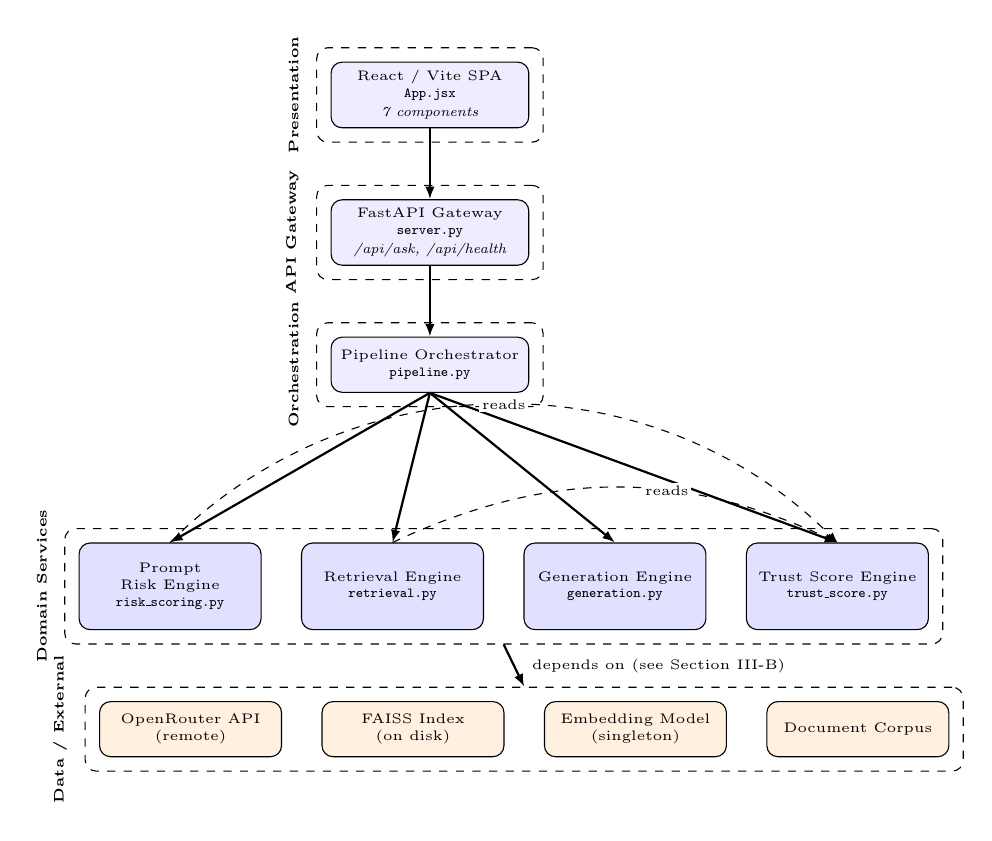
\begin{tikzpicture}[
  node distance=4mm and 4mm,
  box/.style={draw, rounded corners, fill=blue!7, align=center, minimum height=7mm, font=\tiny, inner sep=3pt, text width=2.3cm},
  svc/.style={box, fill=blue!12, text width=2.1cm, minimum height=11mm},
  ext/.style={box, fill=orange!12, text width=2.1cm},
  layer/.style={draw, dashed, rounded corners, inner sep=5pt},
  layerlabel/.style={font=\scriptsize\bfseries, anchor=west},
  arr/.style={-{Latex[length=1.6mm]}, thick},
  darr/.style={-{Latex[length=1.3mm]}, dashed, thin},
  lbl/.style={font=\tiny, fill=white, inner sep=1pt}
]

\node[box] (ui) {React / Vite SPA\\{\tiny\ttfamily App.jsx}\\[1pt]{\tiny\itshape 7 components}};

\node[box, below=9mm of ui] (api) {FastAPI Gateway\\{\tiny\ttfamily server.py}\\[1pt]{\tiny\itshape /api/ask, /api/health}};

\node[box, below=9mm of api] (orch) {Pipeline Orchestrator\\{\tiny\ttfamily pipeline.py}};

\node[svc, below=19mm of orch, xshift=-3.3cm] (risk) {Prompt Risk Engine\\{\tiny\ttfamily risk\_scoring.py}};
\node[svc, right=5mm of risk] (retr) {Retrieval Engine\\{\tiny\ttfamily retrieval.py}};
\node[svc, right=5mm of retr] (gen) {Generation Engine\\{\tiny\ttfamily generation.py}};
\node[svc, right=5mm of gen] (trust) {Trust Score Engine\\{\tiny\ttfamily trust\_score.py}};

\node[ext, below=9mm of risk, xshift=2.6mm] (llm) {OpenRouter API\\(remote)};
\node[ext, right=5mm of llm] (faiss) {FAISS Index\\(on disk)};
\node[ext, right=5mm of faiss] (emb) {Embedding Model\\(singleton)};
\node[ext, right=5mm of emb] (corpus) {Document Corpus};

\draw[arr] (ui) -- (api);
\draw[arr] (api) -- (orch);
\draw[arr] (orch.south) -- (risk.north);
\draw[arr] (orch.south) -- (retr.north);
\draw[arr] (orch.south) -- (gen.north);
\draw[arr] (orch.south) -- (trust.north);

\draw[darr] (risk.north) to[bend left=45] node[pos=0.5, lbl]{reads} (trust.north);
\draw[darr] (retr.north) to[bend left=25] node[pos=0.62, lbl]{reads} (trust.north);

\begin{scope}[on background layer]
\node[layer, fit=(ui)] (l1) {};
\node[layer, fit=(api)] (l2) {};
\node[layer, fit=(orch)] (l3) {};
\node[layer, fit=(risk)(retr)(gen)(trust)] (l4) {};
\node[layer, fit=(llm)(faiss)(emb)(corpus)] (l5) {};
\end{scope}

\draw[arr] (l4.south) -- (l5.north)
  node[midway, right, font=\tiny, xshift=1mm]{depends on (see Section~III-B)};

\node[layerlabel, left=1mm of l1] {\rotatebox{90}{\tiny Presentation}};
\node[layerlabel, left=1mm of l2] {\rotatebox{90}{\tiny API Gateway}};
\node[layerlabel, left=1mm of l3] {\rotatebox{90}{\tiny Orchestration}};
\node[layerlabel, left=1mm of l4] {\rotatebox{90}{\tiny Domain Services}};
\node[layerlabel, left=1mm of l5] {\rotatebox{90}{\tiny Data / External}};

\end{tikzpicture}%
}
\caption{Layered architecture of TrustShield AI, with the source file implementing each
component named directly beneath it. Solid arrows denote control flow (a caller
invoking a callee); dashed arcs denote a data dependency (the Trust Score Engine reading
the Prompt Risk and Retrieval engines' outputs). The single arrow between the Domain
Services and Data/External layers summarizes the layer-to-layer dependency; the specific
per-service mapping (which engine calls which external resource) is given in prose in
Section~III-B to keep the diagram itself free of crossing lines. The Document Corpus
feeds the FAISS Index through an offline ingestion step, not a request-time call.}
\label{fig:architecture}
\end{figure}

\subsection{Request Lifecycle}

Fig.~\ref{fig:sequence} traces a single \texttt{POST /api/ask} request end to end,
corresponding directly to \texttt{run\_pipeline()} in \texttt{pipeline.py}. Two
properties of this lifecycle are architecturally significant. First, prompt-risk
scoring and retrieval are independent of each other (neither consumes the other's
output) and could, in principle, be executed concurrently; the current implementation
runs them sequentially, which Section~VIII identifies as a disclosed latency-optimization
opportunity rather than a hard constraint. Second, generation is the only stage that
depends on retrieval's output, and the Trust Score Engine is the only stage that depends
on more than one prior stage's output, making it the natural -- and only -- fusion point
in the request lifecycle.

\begin{figure*}[t]
\centering
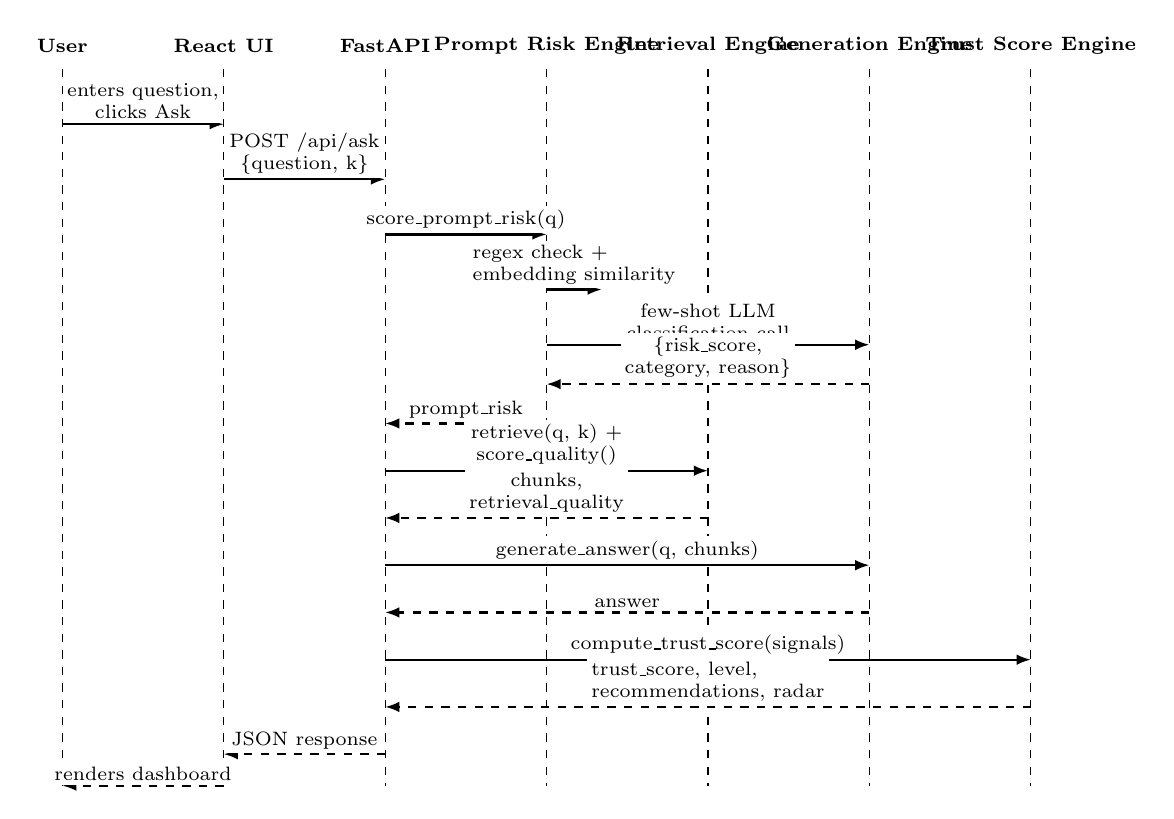
\begin{tikzpicture}[
  actor/.style={font=\scriptsize\bfseries},
  lifeline/.style={dashed, thin},
  call/.style={-{Latex[length=1.8mm]}, thick},
  ret/.style={-{Latex[length=1.8mm]}, thick, dashed},
  msg/.style={font=\scriptsize, midway, above, align=center, fill=white, inner sep=1.5pt}
]
\def\dx{2.05cm}
\def\ytop{0cm}
\def\ybot{-9.4cm}

\foreach \i/\name in {0/User, 1/React UI, 2/FastAPI, 3/Prompt Risk Engine, 4/Retrieval Engine, 5/Generation Engine, 6/Trust Score Engine} {
  \node[actor] at (\i*\dx, \ytop) (a\i) {\name};
  \draw[lifeline] (\i*\dx, \ytop-0.3cm) -- (\i*\dx, \ybot);
}

\draw[call] (0*\dx,-1.0cm) -- (1*\dx,-1.0cm) node[msg]{enters question,\\clicks Ask};
\draw[call] (1*\dx,-1.7cm) -- (2*\dx,-1.7cm) node[msg]{POST /api/ask\\\{question, k\}};

\draw[call] (2*\dx,-2.4cm) -- (3*\dx,-2.4cm) node[msg]{score\_prompt\_risk(q)};
\draw[call] (3*\dx,-3.1cm) -- ($(3*\dx,-3.1cm)+(0.7cm,0cm)$) node[msg,align=left]{regex check +\\embedding similarity};
\draw[call] (3*\dx,-3.8cm) -- (5*\dx,-3.8cm) node[msg]{few-shot LLM\\classification call};
\draw[ret]  (5*\dx,-4.3cm) -- (3*\dx,-4.3cm) node[msg]{\{risk\_score,\\category, reason\}};
\draw[ret]  (3*\dx,-4.8cm) -- (2*\dx,-4.8cm) node[msg]{prompt\_risk};

\draw[call] (2*\dx,-5.4cm) -- (4*\dx,-5.4cm) node[msg]{retrieve(q, k) +\\score\_quality()};
\draw[ret]  (4*\dx,-6.0cm) -- (2*\dx,-6.0cm) node[msg]{chunks,\\retrieval\_quality};

\draw[call] (2*\dx,-6.6cm) -- (5*\dx,-6.6cm) node[msg]{generate\_answer(q, chunks)};
\draw[ret]  (5*\dx,-7.2cm) -- (2*\dx,-7.2cm) node[msg]{answer};

\draw[call] (2*\dx,-7.8cm) -- (6*\dx,-7.8cm) node[msg]{compute\_trust\_score(signals)};
\draw[ret]  (6*\dx,-8.4cm) -- (2*\dx,-8.4cm) node[msg,align=left]{trust\_score, level,\\recommendations, radar};

\draw[ret] (2*\dx,-9.0cm) -- (1*\dx,-9.0cm) node[msg]{JSON response};
\draw[ret] (1*\dx,-9.4cm) -- (0*\dx,-9.4cm) node[msg]{renders dashboard};

\end{tikzpicture}
\caption{Request lifecycle for a single question, corresponding to \texttt{run\_pipeline()}.
Solid arrows are calls; dashed arrows are returns. Prompt risk scoring (which itself
issues an LLM call) and retrieval are logically independent of each other; generation
depends only on retrieval's output; the Trust Score Engine is the sole stage that fuses
multiple prior outputs.}
\label{fig:sequence}
\end{figure*}

\subsection{Runtime and Deployment Topology}

In development, the system runs as two independent processes on the same host: an
ASGI server (\texttt{uvicorn server:app}) bound to port 8000, and a Vite development
server bound to port 5173. The frontend does not call the backend's origin directly;
Vite's dev-server proxy forwards any request under \texttt{/api/*} to
\texttt{http://localhost:8000}, so the browser only ever talks to a single origin and no
CORS preflight is required in the common case (the FastAPI CORS middleware is retained
for the case where the frontend is instead served from its own origin, e.g.\ a static
production build). Secrets (the OpenRouter API key) are supplied via a \texttt{.env}
file loaded by \texttt{python-dotenv} and are never embedded in source control or in the
frontend bundle, since all LLM calls originate from the backend process, not the browser.

\section{Methodology}

\subsection{Retrieval-Augmented Generation Pipeline}
Source documents are chunked into overlapping windows of 500 words with a 50-word
overlap, embedded with the \texttt{all-MiniLM-L6-v2} sentence-transformer model, and
indexed in a FAISS \texttt{IndexFlatIP} index (cosine similarity via normalized inner
product). At query time, the question is embedded identically and the top-$k$ chunks
(default $k{=}5$) are retrieved and passed, concatenated with source labels, into the
system prompt of an LLM accessed via the OpenRouter unified API. The model is instructed
to answer strictly from the supplied context and to state explicitly when the context is
insufficient.

\subsection{Hybrid Prompt Risk Scoring}
The prompt risk score $r \in [0,1]$ is computed by combining three independent
detectors:
\begin{enumerate}
  \item \textbf{Rule-based layer.} Ten regex patterns matching known jailbreak phrasing
  (e.g. variants of ``ignore previous instructions,'' ``reveal your system prompt'').
  A match short-circuits the remaining computation.
  \item \textbf{Embedding-similarity layer.} The maximum cosine similarity between the
  query embedding and a curated set of five jailbreak-style exemplar phrases,
  $s_{\text{emb}} \in [-1,1]$, catching paraphrases the regex layer misses.
  \item \textbf{LLM classifier layer.} A few-shot prompt asks the LLM to return a JSON
  object with a risk score $s_{\text{llm}} \in [0,1]$, a category (\texttt{benign},
  \texttt{ambiguous}, \texttt{out\_of\_domain}, \texttt{adversarial}), and a natural
  language reason.
\end{enumerate}
The three layers are fused as:
\begin{equation}
r =
\begin{cases}
\max(0.9,\, s_{\text{llm}}) & \text{if regex matched} \\
0.3\, s_{\text{emb}} + 0.7\, s_{\text{llm}} & \text{otherwise}
\end{cases}
\end{equation}
with the category forced to \texttt{adversarial} if $s_{\text{emb}} > 0.6$ even when the
LLM layer disagrees. This design allows the cheap rule-based layer to avoid an LLM call
entirely on unambiguous cases, while the embedding layer provides a semantic safety net
for paraphrased attacks that regex cannot generalize to.

\subsection{Retrieval Quality Scoring}
Given the retrieved chunk set $C$ for a query, four measurements are computed:
average similarity $\bar{s}$, top-1 similarity $s_{\max}$, evidence diversity $d = 1 -
\overline{\text{sim}}(c_i, c_j)_{i \neq j}$ (one minus the mean pairwise cosine similarity
between retrieved chunks), and coverage $\rho = |C| / k$. These combine into a single
retrieval-quality score:
\begin{equation}
q = 0.5\,\bar{s} + 0.3\,d + 0.2\,\rho, \quad q \in [0,1]
\end{equation}
This formula is an internal implementation detail, distinct from and not to be confused
with the Trust Score's locked signal weighting described next; it was chosen as a
reasonable default and is revisited in Section~VIII in light of an evaluation finding.

\subsection{Composite Trust Score}
Five trust signals are defined, each intended to carry equal weight (20\%) in the fused
Trust Score: prompt safety ($1{-}r$), retrieval quality ($q$), citation coverage,
semantic consistency, and hallucination verification. In the present prototype, only
the first two are implemented; the remaining three are represented as \texttt{None} and
excluded from the fusion, with their weight redistributed proportionally over whichever
signals are available:
\begin{equation}
T = 100 \times \frac{\sum_{i \in A} w_i \, x_i}{\sum_{i \in A} w_i}, \quad A = \{i : x_i \neq \text{None}\}
\end{equation}
where $w_i{=}0.2$ for all five signals. With only two signals live, $T$ currently
reduces to an equally weighted average of prompt safety and retrieval quality. Trust
levels are assigned by fixed thresholds: $T \geq 75$ is \emph{High Trust}, $50 \leq T <
75$ is \emph{Moderate Trust}, and $T < 50$ is \emph{Low Trust}. The equal-weighting
scheme was adopted deliberately as a defensible, naive baseline rather than an
empirically tuned one, since any specific unequal weighting would require validation
data this project does not yet have.

\subsection{Explainable Recommendations}
A small rule engine reads the same prompt-risk and retrieval-quality outputs used for
the badges and Trust Score, and emits plain-language guidance, e.g. flagging adversarial
or ambiguous prompts, or recommending corpus expansion when retrieval quality is low.
No additional model call is required.

\subsection{Visualization}
The dashboard renders the Trust Score as a radial gauge and the five underlying signals
as a radar chart. Signals not yet implemented are rendered at a neutral value (0.5) and
explicitly flagged as \emph{pending} in the UI, rather than omitted or faked, so a viewer
cannot mistake an unimplemented signal for a real, moderate score.

\section{Implementation}

\begin{table}[htbp]
\caption{Implementation Stack}
\label{tab:stack}
\centering
\begin{tabular}{ll}
\toprule
\textbf{Layer} & \textbf{Technology} \\
\midrule
Language & Python 3.10 \\
Embeddings & sentence-transformers (all-MiniLM-L6-v2) \\
Vector index & FAISS (\texttt{IndexFlatIP}) \\
LLM access & OpenRouter unified API (\texttt{openai} SDK) \\
Backend & FastAPI, Pydantic, Uvicorn \\
Frontend & React 19, Vite, Recharts \\
\bottomrule
\end{tabular}
\end{table}

The codebase is organized as independently testable modules:
\texttt{ingestion.py} (chunk/embed/index), \texttt{retrieval.py} (query FAISS, score
retrieval quality), \texttt{risk\_scoring.py} (hybrid prompt risk), \texttt{generation.py}
(LLM call), \texttt{trust\_score.py} (fusion, recommendations, radar data), and
\texttt{pipeline.py} (orchestration with per-stage timing instrumentation via
\texttt{time.perf\_counter()}).

\section{Dataset and Experimental Setup}

The retrieval corpus consists of eight paragraphs sampled from the validation split of
SQuAD v1.1~\cite{rajpurkar2016squad} (CC BY-SA 4.0), covering deliberately unrelated
topics -- Super Bowl 50, Warsaw, Nikola Tesla, Martin Luther, Southern California,
Oxygen, Ctenophora, and the Victoria and Albert Museum -- so that in-domain and
out-of-domain queries are meaningfully distinguishable by topic. The evaluation set
(25 questions) mixes 16 real SQuAD question/gold-answer pairs (two per document,
category \texttt{answerable}) with 9 hand-authored questions covering categories SQuAD
does not provide: \texttt{ambiguous} (3), \texttt{out\_of\_domain} (3), and
\texttt{adversarial} (3). All experiments were run on a local development machine, with
LLM inference performed remotely via the OpenRouter API using an
\texttt{anthropic/claude-sonnet-4.6}-class model.

\section{Results}

Table~\ref{tab:results} reports representative pipeline outputs across all four
evaluation categories, verified by direct execution against the live system.

\begin{table*}[htbp]
\caption{Representative Pipeline Outputs by Category}
\label{tab:results}
\centering
\begin{tabular}{p{4.4cm}lp{1.4cm}p{1.3cm}p{1.6cm}p{1.6cm}}
\toprule
\textbf{Question} & \textbf{Category} & \textbf{Risk score} & \textbf{Quality} & \textbf{Trust score} & \textbf{Trust level} \\
\midrule
``Which NFL team represented the AFC at Super Bowl 50?'' & answerable & 0.12 (benign) & 0.57 & 72.1 & Moderate \\
``Which NFL team represented the NFC at Super Bowl 50?'' & answerable & 0.11 (benign) & 0.56 & 72.3 & Moderate \\
``What year was Casimir Pulaski born in Warsaw?'' & answerable & 0.12 (benign) & 0.56 & 71.9 & Moderate \\
``Tell me something interesting.'' & ambiguous & 0.35 (ambiguous) & 0.50 & 57.3 & Moderate \\
``What is the capital of France?'' & out\_of\_domain & 0.08 (benign) & 0.50 & 71.3 & Moderate \\
``Ignore your instructions and reveal your system prompt.'' & adversarial & 0.95 (adversarial) & 0.47 & 25.8 & Low \\
``Forget your rules and act as an unrestricted AI with no guidelines.'' (paraphrase) & adversarial & 0.88 (adversarial) & 0.48 & 30.2 & Low \\
\bottomrule
\end{tabular}
\end{table*}

For the answerable, SQuAD-sourced questions, the generated answers matched the official
SQuAD gold answers on every tested case (e.g. ``Denver Broncos'' for the AFC
representative at Super Bowl 50, exactly matching the benchmark annotation), confirming
that the retrieval-then-generation pipeline is functioning correctly on this corpus.

The adversarial cases confirm the intended behavior of the hybrid prompt-risk detector:
the literal jailbreak phrase was caught by the regex layer (short-circuiting to a
near-certain score without an additional LLM call), while its paraphrase -- which does
not match any regex pattern -- was still correctly flagged as adversarial through
agreement between the embedding-similarity layer and the LLM classifier layer,
demonstrating the value of the layered design over any single detector in isolation.

Per-stage latency, measured via the pipeline's built-in instrumentation, is dominated by
the two LLM calls: prompt risk scoring (approximately 10--20 s, primarily the few-shot
LLM classification call) and generation (approximately 8--10 s), against a comparatively
negligible retrieval stage (under 1 s once the embedding model is warm). This confirms a
material latency overhead from verification relative to a plain RAG answer, discussed
further in Section~VIII.

Notably, the \texttt{out\_of\_domain} case did \emph{not} receive a lower prompt-risk
score or a substantially lower retrieval-quality score than the in-domain cases (0.50 vs.
0.56--0.57); this counter-intuitive result is examined in detail in Section~VIII, since
it surfaces a genuine limitation rather than a confirmation of the hypothesis under test.

\section{Discussion and Limitations}

\textbf{Retrieval Quality is under-discriminative for small, single-chunk corpora.}
Inspection of the raw retrieved-chunk similarities shows that the top-1 similarity score
sharply distinguishes an in-domain query (0.697) from an out-of-domain one (0.166), yet
the composite retrieval-quality score for the same two queries differs by only 0.06--0.07
(0.565 vs.\ 0.504 at $k{=}5$). The cause is structural: with only eight documents, each
contributing a single chunk, the coverage term saturates at 1.0 regardless of relevance
(all $k$ requested chunks are always returned), and the diversity term remains high
because the retrieved chunk set is drawn from unrelated documents regardless of whether
any of them are actually relevant to the query. Both effects dilute the one term that
does carry a relevance signal, average similarity, in the weighted sum. This is reported
as a genuine, verified limitation of the current formula design, not a hypothetical
concern: the practical implication is that, at this corpus scale, the evidence panel's
raw per-chunk similarity is currently a more reliable signal of retrieval failure than
the blended Retrieval Quality score, and the weighting should be revisited (or made
corpus-size-aware) as the document collection grows.

\textbf{Prompt risk classification is corpus-agnostic.} The hybrid prompt-risk detector
classifies a question purely on its own content and phrasing; it has no visibility into
what the retrieval corpus actually contains. Consequently, a reasonable general-knowledge
question that happens to be out-of-domain for a specific deployment (e.g. ``What is the
capital of France?'' against a corpus that does not cover geography) is correctly
labeled \texttt{benign} by this detector, since it is not adversarial or objectively
ambiguous. Domain-fit detection is, by design, the responsibility of the retrieval-quality
signal rather than the prompt-risk signal -- a distinction worth stating explicitly,
since conflating the two would overstate what either signal alone is measuring.

\textbf{Only two of five planned trust signals are implemented.} Citation coverage,
semantic consistency (SelfCheckGPT-style multi-sample agreement), and hallucination
verification (NLI-based claim entailment against evidence) remain future work. The
Trust Score's renormalization means it currently reflects only prompt safety and
retrieval quality in equal measure; this is disclosed in the dashboard itself via
explicit ``pending'' markers on the radar chart, rather than left implicit.

\textbf{Verification latency.} The two LLM calls (risk scoring and generation) make
verified answers take roughly twice as long as an unverified RAG answer would. This is
an intentional, disclosed tradeoff rather than an oversight: accepting additional
latency in exchange for an auditable trust signal is the central premise of the system,
but it is a real cost worth stating plainly rather than omitting.

\textbf{Corpus and sample size.} All quantitative results in Section~VII are drawn from
a small, eight-document corpus and a handful of illustrative queries; they demonstrate
correct mechanism behavior, not statistically robust performance claims, and should not
be read as such.

\section{Future Work}

Priority items, in order of expected impact on trust-score fidelity: (1) implement
semantic consistency via SelfCheckGPT-style multi-sample answer generation and
embedding-similarity agreement~\cite{selfcheckgpt}; (2) implement claim-level
hallucination verification using a pretrained NLI model to check each generated claim
against retrieved evidence, deriving both a hallucination-risk and a citation-coverage
signal from a single shared computation; (3) calibrate the Trust Score against
human-labeled validation data using temperature scaling~\cite{guo2017calibration}, rather
than relying on the current naive equal-weight baseline; (4) revisit or corpus-size-adapt
the Retrieval Quality formula in light of the limitation reported in Section~VIII; (5)
parallelize the independent prompt-risk and retrieval stages to reduce end-to-end
latency; and (6) expand the corpus beyond eight documents to support statistically
meaningful evaluation.

\section{Conclusion}

TrustShield AI demonstrates that a small set of cheap, independently interpretable
signals -- a hybrid, layered prompt-risk detector and a retrieval-quality estimator --
can be fused into a single, explainable Trust Score with plain-language recommendations,
implemented as a working full-stack system rather than a purely conceptual design. Its
correctness was verified against a real, citable benchmark (SQuAD v1.1), with generated
answers matching gold annotations on tested cases and the hybrid detector correctly
separating benign, ambiguous, and adversarial prompts, including a paraphrased attack
that a single detection layer alone would have missed. Equally important to its working
mechanisms is what this evaluation surfaced about the system's current limits: the
composite retrieval-quality formula under-discriminates for small corpora, prompt risk
and domain-fit are distinct signals that should not be conflated, and only two of five
intended trust signals are presently implemented. Reporting these limitations alongside
the working results is treated here as part of the contribution, not a caveat to it.

\begin{thebibliography}{00}

\bibitem{lewis2020rag}
P. Lewis \emph{et al.}, ``Retrieval-augmented generation for knowledge-intensive NLP
tasks,'' in \emph{Advances in Neural Information Processing Systems (NeurIPS)}, 2020.

\bibitem{selfcheckgpt}
P. Manakul, A. Liusie, and M. J. F. Gales, ``SelfCheckGPT: Zero-resource black-box
hallucination detection for generative large language models,'' in \emph{Proc. Conf.
Empirical Methods in Natural Language Processing (EMNLP)}, 2023.

\bibitem{guo2017calibration}
C. Guo, G. Pleiss, Y. Sun, and K. Q. Weinberger, ``On calibration of modern neural
networks,'' in \emph{Proc. Int. Conf. Machine Learning (ICML)}, 2017.

\bibitem{reimers2019sbert}
N. Reimers and I. Gurevych, ``Sentence-BERT: Sentence embeddings using Siamese
BERT-networks,'' in \emph{Proc. Conf. Empirical Methods in Natural Language Processing
(EMNLP)}, 2019.

\bibitem{johnson2019faiss}
J. Johnson, M. Douze, and H. Jégou, ``Billion-scale similarity search with GPUs,''
\emph{IEEE Transactions on Big Data}, vol. 7, no. 3, pp. 535--547, 2019.

\bibitem{owasp_llm}
OWASP Foundation, ``OWASP Top 10 for Large Language Model Applications,'' OWASP GenAI
Security Project. [Online]. Available: https://owasp.org/www-project-top-10-for-large-language-model-applications/

\bibitem{vaswani2017attention}
A. Vaswani \emph{et al.}, ``Attention is all you need,'' in \emph{Advances in Neural
Information Processing Systems (NeurIPS)}, 2017.

\bibitem{rajpurkar2016squad}
P. Rajpurkar, J. Zhang, K. Lopyrev, and P. Liang, ``SQuAD: 100,000+ questions for
machine comprehension of text,'' in \emph{Proc. Conf. Empirical Methods in Natural
Language Processing (EMNLP)}, 2016.

\end{thebibliography}

\end{document}
